% !TEX root = NSF_SuperCDMS_SNOLAB_OPS.tex
%% people who build community and knowledge
%% around software?
%% The maintainers
%% Educopia
%% http://ivory.idyll.org/blog/2019-communities-of-effort.html#disqus_thread
%% https://blog.dnanexus.com/2018-01-29-analysis-commons-a-collaborative-approach-to-multi-omics-discovery/

%% describing data
%https://library.si.edu/research/describing-your-data-data-dictionaries
%https://figshare.com/articles/The_State_of_Open_Data_Report_2017/5481187/1
%https://www.usgs.gov/products/data-and-tools/data-management/data-standards
%https://www.fgdc.gov/standards/standards_publications/
%http://www.ddialliance.org/ metadata standards for social sciences
%https://www.rd-alliance.org/groups/data-type-registries-wg.html research data alliance, not focused on physics AFAIK but definitely useful
%https://access-data.trydiscourse.com/
% XDR, external data format!!
% https://tools.ietf.org/html/rfc1832.html#section-6
% and there is a python library for it, xdrlib

% Mom says all the cool kids are using smartsheets
% Liquid Planner has a free plan for teachers?  https://app.liquidplanner.com/space/202855/projects


\subsection{Introduction}

\subsection{Science-driven}
% How will the project outcomes fill well-recognized science and engineering needs of the research community, and advance research capability within a significant area or areas of science and engineering? What are the broader impacts of the project, such as benefits to science and engineering communities beyond initial targets, underrepresented communities, and education and workforce development? The project outcomes should address well-recognized science outcomes.

This project serves the immediate needs of researchers in the dark matter community and the experimental nuclear physics community by providing a common toolset for analyzing data in any format.

The PI expects that

\begin{itemize}
    \item Multiple research projects across the NSF directorate will be more productive because they can use existing, documented tools rather than building their own.  The PI intends to estimate this impact with citations from scientific papers.
    \item Increased involvement of undergraduate researchers in science analysis due to improved documentation and an extended support network.  The PI intends to measure this through undergraduate involvement in her own lab, community surveys, and tracking community forum data.
    \item Several example analyses will be publicly released, with accompanying documentation and support information for pre-requisite computing skills.  The intent is for these educational materials to be accessible to someone with no domain knowledge.  The PI believes these training materials will be an equitable training resource.
\end{itemize}


\subsection{Innovation}
% What innovative and transformational capabilities will the project bring to its target communities, and how will the project integrate innovation and discovery into the project activities, such as through empirical research embedded as an integral component of the project activities? Such research might encompass reproducibility, provenance, effectiveness, usability, and adoption of the components, adaptability to new technologies and to changing requirements, and the development of lifecycle processes used in the project.

A common limitation of data-analysis software that is entirely home-grown is that it does not scale as data grows and changes - a human has to update or rewrite the code if the requirements change substantially.

This library makes heavy use of existing libraries.  The benefit is that as those libraries improve and scale to larger data sets, this software inherits that improvement.  

In both cases, significant human effort is needed to adapt the software to changing data and needs.  But by leveraging well-supported, open-source libraries, the burden is shifted away from an individual scientist and towards an active community that is highly motivated to solve similar problems.  This library serves as sugar to allow scientists with many different data formats to take advantage of these popular libraries.

The danger to this approach is the same - if these libraries lose community support or focus on very different problems then this library will lose relevance over time.  To mitigate this risk, the PI is focusing on integrating with a library supported by the IRIS-HEP collaboration and with pandas, which enjoys extreme popularity in the data science community.

\subsection{Close collaboration among stakeholders}
% How will the project activities engage CI experts, specialists, and scientists and engineers working in concert with the relevant domain scientists and engineers who are users of CI?

The PI proposes to engage both cyberinfrastructure experts and the experimental nuclear physics community by (1) working closely with pilot experiments to build software that works effectively for scientists analyzing event-based data, (2) holding yearly workshops intended to foster interaction between the scientists using the software and cyberinfrastructure developers, and (3) attending conferences that will allow outreach to the scientific community (for example, the Low Energy Community Meeting) and the cyberinfrastructure community (for example, CHEP).

The PI has working relationships with scientists in the SuperCDMS collaboration and the XIA corporation, both of which are interested in exploring the proposed software as solutions to analysis needs.

In addition, the IRIS-HEP collaboration is interested in this work as it would extend their awkward-array library to a broader audience.  Awkward array was developed by Jim as part of DIANA/HEP (http://diana-hep.org,
OAC-1450377) and that effort will continue with IRIS-HEP
(http://iris-hep.org, OAC-1836650).  Collaborating with IRIS-HEP gives us access to experienced cyberinfrastructure developers who have focused on developing software suitable for terabyte-scale data.


\subsection{Building on existing, recognized capabilities}
% How will the project activities build on and leverage existing NSF and national cyberinfrastructure investments, as appropriate?

The proposed work builds on existing capabilities and communities in several ways:

\begin{itemize}
    \item \textbf{The PI proposes to use already-existing data description languages.}  The languages Katai Struct and the Data Format Description Langauage both have active communities and tools that work with data when provided a description.  Kaitai Struct is the target for the proposed work because (1) it is more human-readable than than the XML-based DFDL, and (2) Katai Struct generates code libraries that allow users to load their data into the programming environment of their choice; DFDL currently works by providing an XML or JSON equivalent of the binary data.  While this is a powerful approach because any language with an XML or JSON parser can now read the data, it also produces a secondary data file that is an order of magnitude larger than most binary files.  This makes DFDL, in its current state, unusable for scientists with gigabyte-scale data sets as it would make the required storage space for analysis prohibitively expensive.
    \item \textbf{The PI proposes to use already-existing infrastructure for the data-analysis library.}  Scientists who would like to avoid writing custom software to read their binary data can already use the Kaitai Struct compiler to generate libraries to read their data in python, C++, and a multitude of other languages.  The advantage is that there is substantial support documentation and an active community available for troubleshooting.  The disadvantage is that the current Kaitai Struct python compiler stores the data in a structure that does not provide adequate speed performance for gigabyte-scale data sets.  By improving the existing Katai Struct compiler software, we can build a science-ready analysis library and scientists can benefit from the existing community support and documentation.   
    \item \textbf{Use a supported and optimized data structure}  for the improvements to the Kaitai Struct compiler.  The ``awkward-array'' library was developed by DIANA/HEP and is now supported by IRIS-HEP and is part of a set of libraries designed to provide flexible data-analysis tools for the high-energy physics community.  The awkward-array data structure is optimized for fast queries on an event-based data set and as such is ideal for the majority of nuclear physics data.  By choosing this data structure as the target, we bring the optimized and convenient analysis environment of awkward-array to any scientist who describes their data with the Katai Struct language.
    \item \textbf{Provide analysis tools for the python environment and training materials that take advantage of the python ecosystem.}  Python is a popular analysis environment in the field of big-data and has enjoyed significant adoption in the scientific community; enough so that python support is compiled in the dominant high-energy physics software, ROOT, by default.  By providing a python library for data analysis, scientists can make use of a full ecosystem that supports data analysis: numpy for convenient array manipulation; scipy for fitting; matplotlib for producing publication-quality figures; and even numba for easy compilation of code that needs to run fast.  This entire environment is easily installed - even for users without administration privileges - through the Anaconda Python distribution.  There are many free and paid programming environments that are availble, notably the Jupyter environment.  Code written in this environment is particularly nice as a tutorial because it is rendered nicely on github, gitlab, and interactive notebooks can be opened in one click through binder.  By providing a small set of introductory documentation, scientists can benefit from the effort the python community has put in to lower the barrier for use.
    
\end{itemize}

\subsection{Project plans, and system and process architecture}
% For an "Elements" proposal, the Project Description should include a high-quality management plan. The proposal should include user interactions and a community-driven approach, and provide a timeline including a proof-of-concept demonstration of the key components. Software or data cyberinfrastructure services should be sufficiently described and follow industry best practices, including the architecture of the CI and the engineering process to be used for the design, development, documentation, testing, validation, and release of the software, its deployment and associated outreach to the end user community, and an acceptance and evaluation plan that involves end users. The description of the CI architecture and processes should explain how security, trustworthiness, provenance, reproducibility, and usability will be addressed by the project and integrated into the proposed system and the engineering process, and how adaptability to new technologies and changing requirements will be addressed by the project and built into the proposed system, as appropriate.

The timing of the proposed work is driven by the proposed, yearly workshops that focus on (1) teaching scientists how to use the tools to access their data, (2) working with scientists to perform their analyses in the python environment, (3) identifying improvements needed for the software to be easy to learn and useful in analysis, and (4) bringing developers into close contact with the science community using their tools.  Each workshop will result in an updated roadmap for the software.

Thus, the workshops - and software releases that include testing, documentation, and example analyses - are the primary milestones of the proposed work.

The work for each yearly cycle can be broken down into the following categories: development of basic computing skills learning material; development of the data-access library; planning and execution of the workshop; and a community-driven update of the roadmap.  See Table~\ref{tab:WBS} for details on who will perform this work.

The minimum requirements of the work determine the work plan and are the following:

\begin{enumerate}
    \item If students or staff move on to other positions, their replacements should be able to get up to speed in a month or less.
    \item Someone with no domain knowledge but reasonable persistence should be able to run the example analysis within a week.
    \item Someone with no domain knowledge but reasonable persistence should be able to analyze their own data within a month.
    \item A scientist who uses the access-data library to obtain a science result should know how to cite the software.
    \item A scientist experiencing trouble using the software should be able to determine how to get help quickly (within five minutes of searching).
    \item A scientist who wishes to improve the code should be able to quickly determine how to contact the developers and how to change, test, and push the code.
\end{enumerate}

The scope of the proposed software is relatively modest: copy an existing framework and adapt it so that it stores data in awkward-array structures rather than slower, dictionary structures.  The development and testing of this code will take time - but reference code for similar work exists, there is robust community support, and there is a developer guide that gives specific instructions for developers who wish to extend the existing Kaitai Struct code in this way.  The proposed work is feasible because it connects two libraries that are both designed for this purpose.

The majority of the proposed work is in making this software easy to use for scientists, and making it easy for the community to participate in the direction and development of the software.  This requires robust documentation for both users and developers.  Users will require installation instructions, instructions for using the library, and guidance on how to adapt the examples for their own analysis needs.  Developers will need additional documentation: instructions for changing the code and testing the code, and instructions and guidance on contributing their changes to the project.

To meet the minimum requirements, the workplan involves creating of initial documentation and an automated testing suite by the Professional Research Associate and example analysis created by the Master's student.

Undergraduates will begin either by working on new scientific computation skills or improving or adding to material of already-developed scientific computation skills.  Students who join the lab currently have two first projects to chose from: working through an introductory lab on water simulation, or working through an example analysis of gamma-spectroscopy data.  The students try to perform their work using existing documentation; the PI provides guidance when this is inadequate.  This provides an opportunity for students to design improvements and learn the basics of contributing to a code repository.  In addition to providing valuable training for the students, this process identifies gaps in the documentation that are often invisible to experts.

This initial work is expected to result in improvements and additions to web-accessible tutorial materials.  In addition, this training will provide a foundation that will allow the students to attempt the following actions:

\begin{itemize}
    \item Successfully follow a simple example analysis using the data-access library.
    \item Successfully follow a tutorial to make and share a change to the library documentation.
    \item Successfully follow a tutorial to make, test, and share a change to the library source code.
\end{itemize}

\begin{tabularx}{\textwidth}{XXX}
Work & Who & Notes \\
\toprule
Roadmap \& workplan development
& PI, PRA, Master's student
& \\

Basic skills materials 
& Undergrads
&  \\

Data-access library development
& 
& \\
code dev
& Professional Research Assistant
& this includes testing, user documentation, and dev documentation\\
contributing
& Professional Research Assistant
& this includes automated testing and contribution guidelines and instructions \\
example analyses
& Master's student
& \\
documentation testing
& Undergraduates, Master's student
& documentation testing may feed back into additional skill documetation \\

Workshop
& 
& \\
Recruiting
& PI
& \\
Organization
& Professional Research Assistant, Undergraduates
& \\
Pre-workshop analysis coordination
& PI, Master's student, PRA
& \\

Community-driven update of roadmap
& PI, PRA, Community
& \\
\label{tab:WBS}
\end{tabularx}

\begin{figure}[htb]
    \begin{center}
      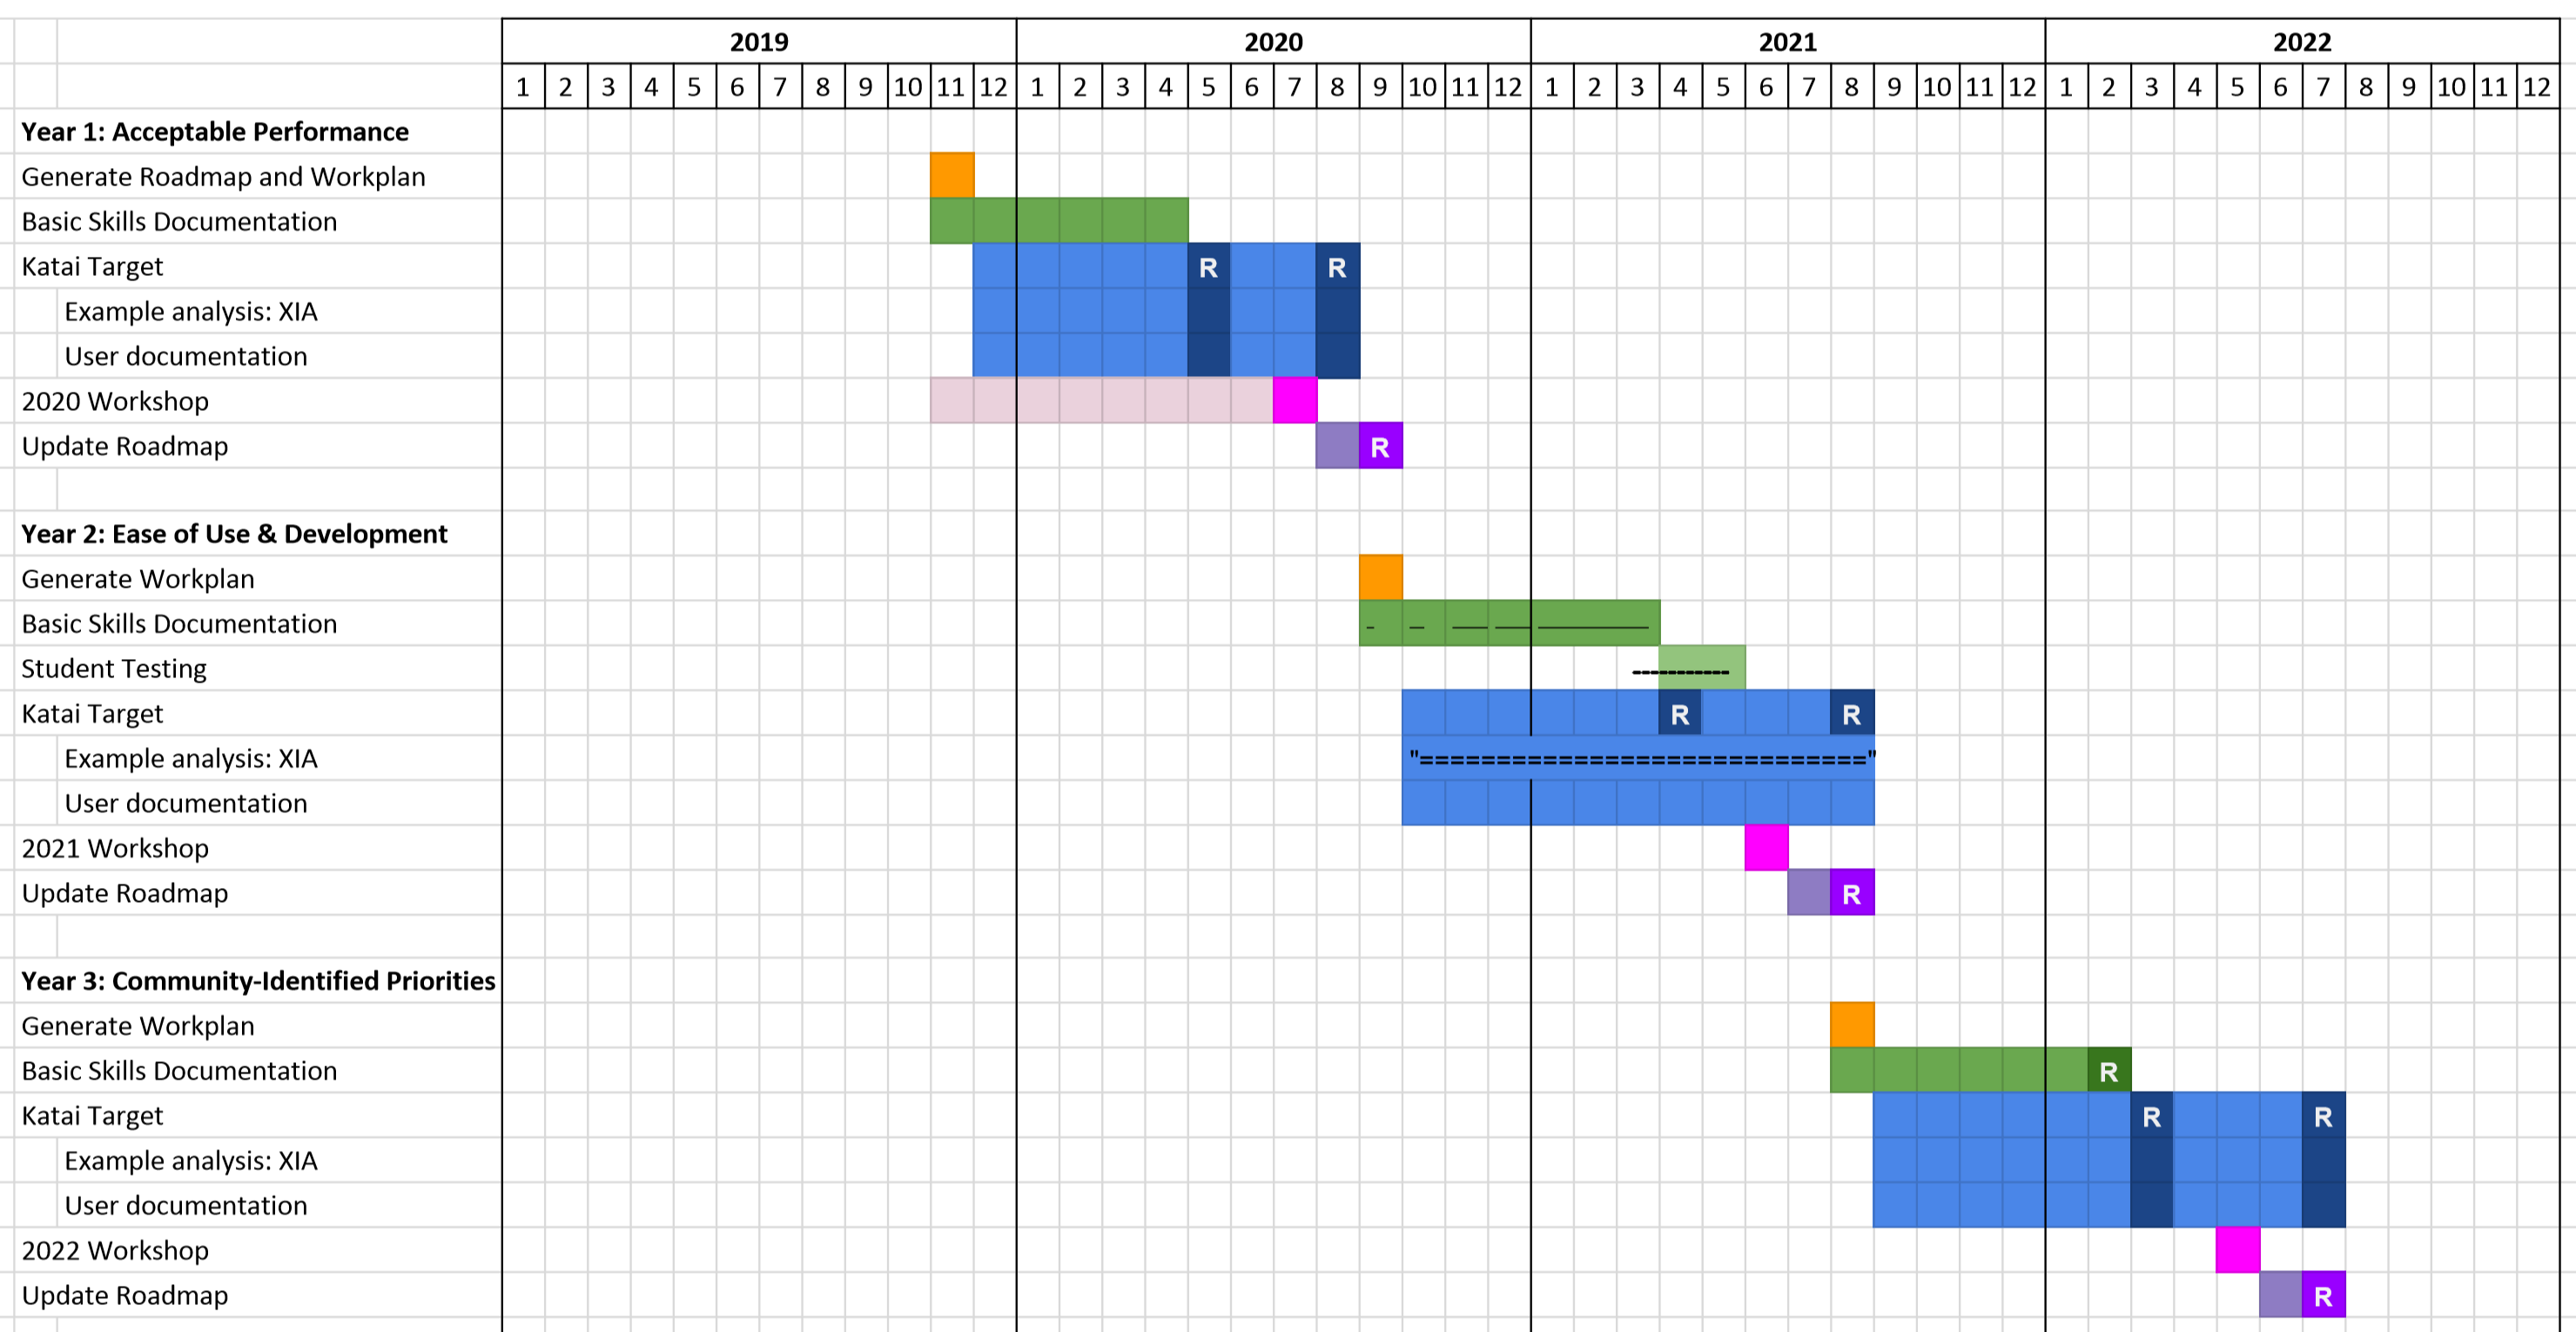
\includegraphics[width=\textwidth]{Figures/schedule1}
    \end{center}
    \caption{Schedule for the proposed work.}
    \label{fig:ops-schedule}
\end{figure}

\textbf{Architecture of the software:}
The architecture of the Kaitai Struct compiler that targets an awkward-array data structure will follow that of the existing Katai Struct software.  Implementing a Kaitai Struct compiler for a new language requires

\begin{enumerate}
    \item Writing a ``runtime library'' that provides a standard stream interface in the target language.  For example, one of the functions every language needs to have defined is a method that returns the size of the file or string stream.  By writing a ``size'' function for the language of interest that follows the Katai Struct API, the code generation becomes simpler.
    \item Writing a ``compiler'' that translates Kaitai Struct concepts, implemented in Scala, into the target language.
    \item Writing a test runner for the new language. 
\end{enumerate}

The proposed work targets the python environment, and there is already a Kaitai Struct python compiler.  The ``compiler'' for the python implementation, however, stores data in native-python data structures that provide inconveniently slow access to standard queries on large, gigabyte-scale data sets.  

However, the changes that need to be implemented to instead store the data in the faster awkward-array data structure are restricted to the compiler code.  The runtime library provides a convenient interface for reading data from a file or stream - this code only cares about the file system interface and does not need to change.  The python test interface will need to be updated as the access syntax for the data will change slightly.

Although there is opportunity for improving the speed of the data load, this development will instead focus on adhering to the existing format and style of Kaitai Struct.  The goal is to make the existing Kaitai Struct community useful to scientists who work with gigabyte-scale data sets; waiting for a few minutes for the data to load is not ideal but is typical of many locally-built solutions.  We can address the more-critical issue of rapid data queries while staying well within the existing framework of Kaitai Struct and intend to do so for the initial implementation of the software.

If we find that data-load times are a significant issue for the nuclear physics community then we will consider more substantial changes to the Kaitai Struct compiler and runtime libary.

\begin{lstlisting}
def size(self):
    # Python has no internal File object API function to get
    # current file / StringIO size, thus we use the following
    # trick.
    io = self._io
    # Remember our current position
    cur_pos = io.tell()
    # Seek to the end of the File object
    io.seek(0, SEEK_END)
    # Remember position, which is equal to the full length
    full_size = io.tell()
    # Seek back to the current position
    io.seek(cur_pos)
return full_size
\end{lstlisting}

\begin{lstlisting}
uint64_t kaitai::kstream::size() {
    std::iostream::pos_type cur_pos = m_io->tellg();
    m_io->seekg(0, std::ios::end);
    std::iostream::pos_type len = m_io->tellg();
    m_io->seekg(cur_pos);
    return len;
}
\caption{The details of this code are not important.  What is significant is the name of this function, size(), and its behavior: find and report the size of the file, without changing where we are in the file.  The Katai Struct compiler for both C++ and python can use the ``size()'' function rather than including these language-specific stream commands, making the compiler code more readable.}
\end{lstlisting}

\textbf{Architecture of the user documentation:} User documentation should make it possible for users with little to no domain knowledge to use the data-access library for science.  Documentation for the use of the library will be stored as text files in the repository with the code.  The files will be written in markdown syntax to improve their readability; this will also render them nicely on cloud-based repository hosts such as github and gitlab.  The following documentation will be provided:

\begin{enumerate}
    \item How to get help with questions or issues about the library.
    \item How to install the library and its dependencies.
    \item An overview explaining what the user will need to provide (data and a description of the data) and what the library will provide (software to read that data).
    \item A tutorial walking through the use-case of a scientist looking at simple data with a custom format.
    \item Links to additional resources detailing more complex data formats and more complex analyses.
    \item Citation guidelines.  
\end{enumerate}


\textbf{Architecture of the developer documentation.}  Documentation intended to facilitate development of the code will be stored in the repository alongside the code.  Text files referenced in the top-level README file will detail, for every repository,

\begin{enumerate}
    \item How to install, develop, and test the code for individuals who wish to make changes.  
    \item How to contribute changes back to the project.  This will provide instructions on the version control practices used by the repository maintainers and instructions for implementing the tests required for changes to be considered for merging with the main code base.
\end{enumerate}

\textbf{Architecture of the basic scientific computing skills documentation:}  Documentation of basic computational skills and concepts will have several possible forms: (1) Text and images, (2) tutorial videos, (3) jupyter notebooks, (4) printable images that illustrate a focused concept, and (5) links to recommended resources such as Software Carpentry tutorials.

All materials will be licensed with  a permissive, open-source license such as CC-BY or MIT.  The source for all the materials will be publicly available through a public host such as github or gitlab and will be archived on a content-tracker such as the Open Science Framework or Figshare.  Videos will be released on YouTube and licensed CC-BY.

All materials will be disseminated using a static site generated by Antora.  Antora is specifically designed for documentation and allows a user to specify a set of repositories containing text files formatted in the Asciidoc markdown language to build a single, searchable documentation site.  Because Antora generates a static site, free hosting services are readily available.  This solution allows my students to focus on creating material to explain core concepts and practice interacting with version control rather than spending time wrestling with web development.

The topics students choose to document are largely student-led, with some guidance from the PI.  Spring 2019 marks the inception of this project, and the concepts chosen by students for illustration have focused on (1) tutorial-format guide for installing python and running a basic python-based analysis of gamma spectroscopy data, (2) instructions for using a docker container to simplify installation of a complex software environment, and (3) a poster explaining what an executable file is.

Documentation that will be provided in this format alongside the scientific computing resources will include

\begin{enumerate}
    \item instructions on where to get help with the material and how to provide feedback and and file bug reports
    \item instructions for those who wish to contribute to the documentation
    \item instructions for the deployment of the documentation
\end{enumerate}


\textbf{Engineering processes:}
% design, development, documentation, testing, validation, and release of the software
% and
% description of the CI architecture and processes should explain how security, trustworthiness, provenance, reproducibility, and usability will be addressed by the project and integrated into the proposed system and the engineering process


\textbf{Deployment and user outreach:}

\textbf{Acceptance and evaluation:}

\textbf{Adaptability:}



\subsubsection{Security}

\subsubsection{Trustworthiness}

\subsubsection{Provenance}

\subsubsection{Reproducibility}

\subsubsection{Usability}

\subsubsection{Adaptability}

\subsection{Deliverables}


\subsection{Metrics}


\subsection{Sustained and sustainable impacts}